\documentclass[titlepage]{article}
\usepackage[left=2.54cm,top=2.54cm,right=2.54cm,nohead]{geometry}
\usepackage{graphicx}
\setlength{\parskip}{2mm}
\title{User Manual for [Product]}
\author{Yubin Kim, Daniel Burstyn, Gobaan Raveendran, Nathaniel Flath}
\begin{document}
\maketitle
\newpage
\tableofcontents
\newpage

\section{Introduction}

\subsection{Outline}

\subsection{Product Overview and Motivation}
\ \ \ \ [Product] at its core is a large system that crawls the internet and
collects blog information.  Blogs in particular are an interesting data source
because, unlike most web pages, they are typically written by a single person
from their point of view.  If we filter out this particular data we can
investigate what the big topics the blogging population (the "blogosphere") is
talking about.

[Product] can be used in two very distinct ways.  The first is its web
interface, which allows users to query the database looking for
\textbf{opinions} on a topic.  A typical Google search will typically return a
wide range of informative results.  However, user will frequently want to hear
about a product or service from another actual person.  [Product] can be used
to find user stories and not just feature lists.

The second use is more advanced and aims to provide access to the collected
data through an API.  This API is available to developers who want to perform
their own analysis on our corpus of blogs.  This saves them the trouble of
having to collect and clean all that data.


\section{Search Basics}
Search is simple: just type whatever comes to mind in the search box, hit
Enter or click on the Search button, and [Product] will search the
blogosphere for blogs that are relevant to your query.  Unfortunately, due to
the nature of natural languages, it may be hard to get exactly the results you
were looking for without refinement. Thus, the following tips can help you
refine your technique to make the most of your searches.

\subsection{Some Basic Facts}
\begin{itemize}
\item \textbf{Select a category.} Certain terms in natural languages become
almost impossible to disambiguate, for example logs about opera's can either
be about the theatrical performances, or the browser, or many other words.
Furthermore, results can be obtained faster and more filter functions can be
used when a category is selected, due to the nature of the search algorithms
used by [Product].
\item Search is always case insensitive. Searching for “new york times” is the
same as searching for “New York Times”.
\end{itemize}

\subsubsection{How to read search results}
[Product]'s goal is to provide you with results that are clear and easy to
read. The diagram below points out four features that are important to
understanding the search results page:
\begin{center}
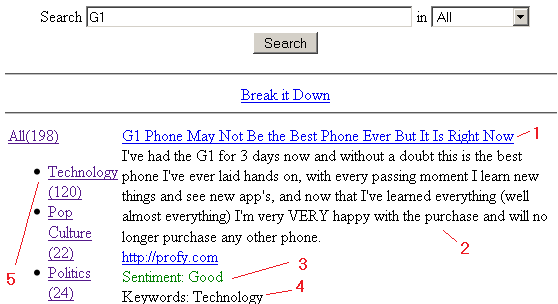
\includegraphics{results.png}
\end{center}

\begin{enumerate}
\item The Title: The first line of any search result is the title of the
webpage.
\item The Snippet: A description of or an excerpt from the webpage.
\item The Sentiment: The basic stance the article has about the topic.
\item Keyword: The category this blog falls under.
\item Bins: Summary of categories for each result.
\end{enumerate}

All these features are important in determining whether the page is what you
need. The title is what the author of the page designated as the best short
description of the page.

The snippet is [Product]'s algorithmic attempt to extract just the part of the
page most relevant to your query. The sentiment plus keywords help you figure
out if the article is what you want. Keywords help you verify that the link is
the correct topic, and the bins will allow you to refine the results if you
find that there are to many options, and many are irrelevent.

\subsection{Break it down}
If a finer level of detail is wanted, press “Break it down”.This mode causes
all the data to be split into organized into good and bad results. This allows
you to gather a quick overview of the system, and get an overall idea of how
positive and negative the results are.

\subsubsection{How to read the breakdown}
The following screen helps us determine how the breakdown works in order to
get a quick overview of the system.
\begin{center}
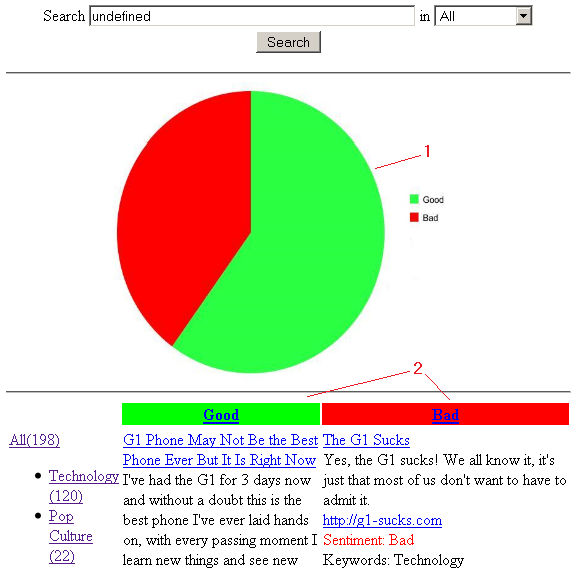
\includegraphics{brokendown.png}
\end{center}

The breakdown consists of two components:
\begin{enumerate}
\item Visualization
\item Result separation.
\end{enumerate}

The visualization component consists of a simple pie graph that will allow you
to quickly determine if the overall sentiment is pro or against the given
topic.  The separation component allows us to isolate one set of opinionated
results, and by clicking a sentiment we can display only the results that
match the sentiment.


\subsection{Help Mode}
Users can get help with our product by clicking a `help' link on any of our
pages.  This link redirects to help on the page they just came from; if
clicked on our main page, it will explain the purpose of our product and how
to use it.  This `main' help page will also be accessible from all other help
pages.  If `help' is clicked on a results page, the opened page will also
explain how to interpret the results presented.

    TODO: screenshot

The above screenshot shows the main help page.  As described previously, it
has basic information about our product and how to use it.  It additionally
links to this document, or an updated user manual.  The help navigation tree
is on the left, allowing the user to easily access help on any feature they
desire.

    TODO: mock-up screenshots of help page

The above screenshot shows a sample help web page for an analysis page.  As
you can see, each feature on the page has an explanation---the visualization
explains how the data was broken down, each column of data has an explanation
describing it, etc.  This page describes to the user precisely what they are
looking at and what they can do in order to clear any confusion they may
have.

\section{Advanced Features}
\begin{itemize}
\item insert blurb here about the fact that we provide APIs and what situation
they can be used
\end{itemize}

\subsection{Data Access API}
The Data Access API allows developers to get direct access to [Product]'s
database of blog information.

\subsection{Sentiment Search API}
The Sentiment Search API has the exact same function as [Product]'s web
interface but can be accessed programmatically.  This is useful for advanced
users that wish to retrieve blog post information and do their own analysis on
top of to existing sentiment analysis.

\section{Glossary}
\begin{description}
\item[Blogosphere] 
The blogosphere is made up of all blogs and their interconnections. The term
implies that blogs exist together as a connected community (or as a collection
of connected communities) or as a social network in which everyday authors can
publish their opinions.
\item[API]
API stands for Application Programming Interface and is an interface that a
piece of software implements that allows other software to interact with it.
\end{description}
\end{document}

